\documentclass[12pt]{article}
\usepackage[left=3cm, right=3cm, top=2cm]{geometry}
\usepackage{graphicx}
\usepackage{fancyhdr}
\usepackage{algorithm}
\usepackage{algorithmic}
\usepackage{listings}
\usepackage{hyperref}
\usepackage{enumitem}
\usepackage{tabularx}
\usepackage{ragged2e}


\hypersetup{colorlinks,linkcolor=black,citecolor=black,filecolor=black,linkcolor=black,urlcolor=black}
\title{Project}
\author{mithu}
\date{ }
\linespread{1.3} 


\begin{document}
\newenvironment{changemargin}[3]{%
\begin{list}{}{%
\setlength{\topsep}{0pt}%
\setlength{\leftmargin}{#1}%
\setlength{\rightmargin}{#2}%
\setlength{\listparindent}{\parindent}%
\setlength{\itemindent}{\parindent}%
\setlength{\parsep}{\parskip}%
}%
\item[]}{\end{list}
}

\newenvironment{boxed}[1]
    {
	\pagenumbering{roman}
      
    }





\vspace*{0.001cm}
\begin{center}\large \textbf{A CRYPTOCURRENCY WALLET}
 \end{center} 
\vspace{0.17cm}
 \begin{center}\textbf{A PROJECT REPORT}\end{center}
\vspace*{0.001cm}
\begin{center}submitted by\end{center}
\vspace*{0.001cm}
\begin{center}
\begin{tabular}{l l}
\bf{HAWA AFLINA} & \bf{DMC18CS015} \\
\bf{MUHAMMAD MIDLAJ} & \bf{DMC18CS017} \\
\bf{MUHAMMED NUAMAN SADIQ} & \bf{DMC18CS018} \\
\bf{SHELGA SHABOOM} & \bf{DMC18CS022} \\

\end{tabular}
\end{center}
\vspace*{0.001cm}
\begin{center}\bf{To} \end{center}
\vspace*{0.001cm}
\begin{center}The APJ Abdul Kalam Technological University \\
In partial fulfillment of the requirements for the award of the Degree\end{center}
\vspace{0.001cm}
\begin{center}Of\end{center}
\vspace*{0.001cm}
\begin{center}Bachelors of Technology \\ In\\
\emph{Computer Science and Engineering}\end{center}

\begin{figure}[H]
\begin{center}

\includegraphics[scale=.5]{MDIT1}
\end{center} 
\end{figure}
\vspace{0.001cm}
\thispagestyle{empty}
\begin{center}\large \bf{M Dasan Institute of Technology (MDIT) \\
Ulliyeri P.O, Kozhikode-673620} \end{center}
\vspace*{0.001cm}
\begin{center}Department of Computer Science and Engineering \end{center}
\vspace{0.001cm}
\begin{center}MAY 2022\end{center}


















\newpage

\begin{boxed}{Title of the Box}


\vspace*{30px}
\begin{center}\LARGE\bf{DECLARATION}\end{center}

We undersigned declare that the project report “A CRYPTOCURRENCY WALLET”, submitted for the partial fulfillment of the requirements for
the award of the degree of the Bachelors of Technology under the university of
the APJ Abdul Kalam Technological University, Kerala is a bonafide work,
done by us under the supervision of the Ms.Ambili Antharjanam (Asst Prof). This
submission represents our ideas in our own words and where ideas or words
of others have been included; We have adequately and accurately cited and
referenced the original sources. We also declare that we have adhered to ethics
of academic honesty and integrity and not misrepresented or fabricated any
data or idea or fact or source in our submission. We understand that any
violation of the above will be a cause for disciplinary action by the
institute and the university and can also be evoke penal action from the sorce
which has thus not been properly cited or from whom proper permission has
not been obtained. This report has not been previously formed the basis for
the award of any degree, diploma or similar title of any other university.
\\Place :
\\Date :
\\
\\
\\
\\
\\
\\
\\
\begin{center}HAWA AFLINA\end{center}\vspace{-6mm}
\begin{center}MUHAMMAD MIDLAJ\end{center}\vspace{-7mm}
\begin{center}MUHAMMED NUAMAN SADIQ\end{center}\vspace{-7mm}
\begin{center}SHELGA SHABOOM\end{center}\vspace{-7mm}



\thispagestyle{empty}

\newpage
\vspace*{1px}
\begin{center}\large\bf{M.DASAN INSTITUTE OF TECHNOLOGY}\end{center}
\begin{center}\large\bf{ULLIYERI} \end{center}
\begin{center}Approved by AICTE, New Delhi \& Affiliated to APJ Abdul Kalam Technological University\end{center}
\begin{center}(KTU)\end{center}

\begin{figure}[H]
\begin{center}

\includegraphics[scale=.4]{MDIT1}
\end{center} 
\end{figure}
\begin{center}\LARGE\bf{CERTIFICATE} \end{center}
\vspace{5mm}
\justifying
This is to certify that the report entitled “A CRYPTOCURRENCY WALLET” by “HAWA AFLINA” (DMC18CS015), “MUHAMMAD MIDLAJ” (DMC18CS017), “MUHAMMED NUAMAN SADIQ“ (DMC18CS018)and “SHELGA SHABOOM” (DMC18CS022) to the APJ Abdul Kalam Technological University in partial fulfillment of the requirements for the award of the Degree of Bachelors of Technology in Computer Science Engineering is a bonafide of seminar carried by his under our guidance and supervision. This report in any form not been submitted to any other University or Institute of any purpose.
\thispagestyle{empty}
\begin{center}
\begin{tabularx}{1\textwidth} { 
  >{\raggedright\arraybackslash}X 
   >{\raggedright\arraybackslash}X 
   >{\raggedright\arraybackslash}X }
 
\\  \\ \\ 

Project Guide & Project Coordinator & Head of The Department  \\  
Ms. AMBILI ANTHARJANAM  & Ms. RAMITHA  M A & Ms. NITHYA V P \\ 
Asstistant Professor  & Asstistant Professor &Asstistant Professor \\ 
Dept. of CSE & Dept. of CSE & Dept. of CSE   











\end{tabularx}
\end{center}


















\newpage
\vspace*{50px}
\begin{center}\LARGE\bf{ACKNOWLEDGEMENT}\end{center}

\thispagestyle{empty}We would like to thank THE ALMIGHTYs mercy towards us over the years;
it goes without saying that without them, We would not be where we are today. \\
\par We would like to place on record, sincere thanks to all those who have
contributed to the successful completion of this project\\
\par We recollect with of gratitude the valuable guidance and the whole hearted support of \textbf{Ms. Ambili antharjanam } (Asst Prof) Department of CSE our internal guide. We are very grateful to our project Coordinator\textbf{ Ms. Ramitha M A} (Asst Prof) and the Head of the department\textbf{ Ms. Nithya V P}, CSE Department for their valuable suggestions throughout the project work\\
\par We wish to express the deep sense of gratitude and the thanks to the Principal \textbf{Mr. Maheesan P M} and Director\textbf{ Mr. H. Ahinus} for the excellent facilities and continual support provided during the course study and project work. \\
\par We thank all the staff members of Computer Science and Engineering Department for their valuable suggestions. \\
\par We also thank all beloved friends for their encouragement, timely help and suggestions.\\

\newpage
\vspace*{50px}
\begin{center} \large \bf{ABSTRACT} \end{center}
               
\vspace{30px}
—A blockchain is a growing list of records, 
called blocks, that are linked using cryptography. 
Blockchain private and public keys are stored in a 
cryptocurrency wallet, but not the actual currency 
values. Wallets provide customers with the ability to 
send and receive virtual currency / tokens and tune their 
balance through interaction with blockchains. Multicurency wallets may be broken down into 3 categories: 
software, hardware, and paper. Software wallets are 
web, mobile and desktop.Cryptocurrency wallets (crypto-wallets) are key to use
blockchain. Every user, who intend to use blockchain
platform for any transaction, has to use crypto-wallet.
Unlike traditional pocket wallets, cryptocurrencies are not
stored in crypto-wallets. Growing penetration of 
blockchain in many industries makes one to understand 
wallets in detail. There are a variety of wallet kinds to 
pick out from. This paper focuses on multi-currency 
wallets review exploring on features like supported 
currencies, anonymity, cost, platform support, key 
management, wallet recovery methods and fiat 
currencies supported.

\newpage
\tableofcontents
\clearpage
\listoffigures
\clearpage
\renewcommand{\headrulewidth}{0.0pt}
\pagestyle{plain}

\end{boxed}
\pagestyle{fancyplain}




\newpage



\thispagestyle{plain}

\pagestyle{plain}
\lhead{A Project Name}
%\chead{}
\rhead{Project Report 2021}
\lhead{A Cryptocurrency Wallet}
\lfoot{Department of CSE}
\cfoot{\thepage}
\rfoot{M-DIT Kozhikode}


%\pagestyle{plain}
%\pagenumbering{arabic}
%\pagestyle{fancy}
%\fancyhf{}
%\fancyhead[LE,RO]{Seminar Report 2021}
%\fancyhead[RE,LO]{ U.S Pandemic prediction using regression and neural network}
%\fancyfoot[LE,RO]{Department of CSE}
%\fancyfoot[CE,CO]{\thepage}
%\fancyfoot[RE,LO]{M-DIT Kozhikode}

\pagenumbering{arabic}

\begin{flushleft}\textbf{CHAPTER 1} \end{flushleft}
\begin{flushleft}\section{INTRODUCTION} \end{flushleft}
   Blockchain software is an immutable database with 
secured access by design. It is an open, distributed ledger 
that can record transactions, which are verifiable, between 
parties effi-ciently. A blockchain is commonly managed 
through a peer-to-peer network forming a disbursed ledger, 
all peers together ad-here to a protocol for inter-node 
communication and vali-dation of new blocks. A valid data 
is recorded on blockchain with consensus of network and 
linked with hash of previous blocks thus it becomes 
immutable record. Hence, a recorded block can’t be altered 
retroactively without alteration of all next blocks. Although 
blockchain statistics are unalterable, blockchains could also 
be taken into consideration steady by layout and exemplify a 
disbursed computer gadget with high Byzantine fault 
tolerance. Cryptocurrency wallets (crypto-wallets) are key to use 
blockchain. Every user, who intend to use blockchain 
platform for any transaction, has to use crypto-wallet. 
Unlike traditional pocket wallets, cryptocurrencies are not 
stored in crypto-wallets. In fact, cryptocurrencies are neither 
stored in any single area nor exist anywhere in any bodily 
form, but it exists as data of transactions stored on 
blockchain. Wallets facilitate user to create an account, i.e., 
a pair of private key and public key and store it in a wallet 
software. To make any transaction on the blockchain, a user 
has to sign off his possession of the coins to his wallet’s 
address. User can spend coins by unlocking the funds in the 
wallet using keys stored in the wallet. There is no realexchange of actual coins, but the exchange of transaction 
data values is created at the blockchain. Thereby, a trade of 
balance in customers crypto-wallet.Cryptocurrency wallet is much more secure than the 
exchanging. A long string, which is referred to as the key 
represents the address of your portfolio and generated 
through sophisticated cryptography techniques. 

\newpage
  Wallets are commonly known as software or hardware
wallets. Soft wallets are downloadable software programs
for your PC or phone, while hardware wallets are physical
vaults that store cryptocurrency data on a specially designed
hard drive contained in the device. Soft wallets are typically
hot or cold. Hot wallet: A wallet is hot when it’s connected
to the Internet. Nothing on the Internet is 100\% secure, so
funds kept in a hot wallet are always at a slight risk of theft
or loss from software bugs. Cold wallet: A wallet is cold
when it’s safely offline and can’t be deliberately or
accidentally compromised over the Internet. All the popular
hardware wallets are designed to be as secure as possible
and can be backed up in different ways. \par
Digital wallets are not registered under the law of any
country, so it is important to cautiously choose the
cryptocurrency wallet for digitized transactions. It is always
better to choose a universal cryptocurrency wallet that
supports more than one cryptocurrency. \par
Wallets are software applications which can be used to
view cryptocurrency balances and make transactions. Each
wallet type is a piece of different software, which provides
access to blockchain data and operate on blockchain data. In
general, any given wallet can work with one or more
cryptocurrencies and features. Public addresses are like
cryptocurrency precise account numbers, they are used to
acquire a particular kind of cryptocurrency and can be
shared publicly. For example, to access Bitcoin blockchain
one needs Bitcoin address, similarly to access Ethereum
blockchain one needs Ethereum address. Wallet helps to
access all transactions associated with that address on
respective blockchain. In general, a wallet allows you to
view balances associated with an address and lets you move
funds around on the blockchain till you are the owner of the
address.
\newpage


\begin{flushleft}\textbf{CHAPTER 2}\end{flushleft}
\begin{flushleft}\section{LITERATURE REVIEW}\end{flushleft}
\vspace*{10px}
\subsection{Wallet Contracts on Ethereum}

   On the blockchain, cryptocurrencies play a role
similar to cash, while cryptographic tokens are a universal
tool for handling rights and assets. Software wallets interact
with blockchains in general and with smart contracts (on-chain
programs) in particular. Some wallets are realized (partly) as
smart contracts with the intent to increase trust and security
by being transparent and by offering features like daily limits,
approvals, multiple signatures, and recovery mechanisms.
Ethereum is the most prominent platform for both, tokens
and smart contracts, and thus also for wallet contracts. We
discuss several methods for identifying wallet contracts in a
semi-automatic manner by looking at the deployed bytecodes
and their interaction patterns. Furthermore, we differentiate
characteristics of wallets in use, and group them into six types.

\subsubsection{Introduction}

\par 
Wallets keep valuables, credentials, and items for access
rights (like cash, licenses, credit cards, key cards) in one place,
for ease of access and use. In this paper, we investigate wallet
contracts on the main chain of Ethereum qualitatively as well
as quantitatively up to block 8 450 000, mined on August 30,
2019. An extended version of this work can be found at [1].
Methodologically, we start from the source code of wallets
and determine characteristic functions. Then we search the
deployed bytecode for variants of the wallets with the same
profile. Some wallets can also be detected by their creation
history or by the way they interact with other contracts. We
group the wallets according to their functionality and collect
creation and usage statistics from the blockchain data. In total,
we found 3.9 M deployed wallet contracts of different 24 types.
This work thus contributes to a better understanding of what
smart contracts on Ethereum are actually used for. We extract
a comprehensive collection of blueprints for wallet contracts
and thereby compile a ground truth. Moreover, the wallet
blueprints and the features they implement may serve as a
resource when designing further decentralized trading apps.

\newpage

\subsubsection{Working}

1) Code Skeletons: To detect functional similarities between contracts we compare their skeletons. These are obtained from the bytecodes of contracts by replacing metadata, constructor arguments, and the arguments of PUSH
operations uniformly by zeros and by stripping trailing zeros.
The rationale is to remove variability that has little impact
on the functional behavior, like the swarm hashes added by
the Solidity compiler or hard-coded addresses of companion
contracts. Skeletons allow us to transfer knowledge gained
about one contract to others with the same skeleton. Note
that the 18 M contract deployments so far give rise to 252 k
distinct bytecodes and just 119 k distinct skeletons. While
only 77 k (0.4 \%) contracts provide verified source codes on
etherscan.io, we are able to relate 6.7 M (37 \%) of the
contracts to corresponding verified source code by exploiting
creation histories and the similarity of skeletons.
\\
2) Interface Extraction: We developed a pattern-based tool
to extract the interface contained in the bytecode. As ground
truth for validation, we used the 77  verified source codes
together with the corresponding bytecode and ABI as provided
by Etherscan. The signatures extracted by our tool differed
from the ground truth in 42 cases. Manual inspection revealed
that our tool was correct also in these cases, whereas the ABIs
did not faithfully reflect the signatures in the bytecode (e.g.
due to compiler optimization or library code).
\\
3) Interface Restoration: To understand the purpose of
contracts we try to recover the function headers from the
signatures. As the signatures are partial hashes of the headers,
we use a dictionary of headers with their 4-byte signatures
(collected from various sources), which allows us to obtain a
header for 59 \% of the 254 k distinct signatures on the main
chain. Since signatures occur with varying frequencies and
codes are deployed in different numbers, this ratio increases
to 89 \% when picking a deployed contract at random.
\par
They define a wallet as a contract that only manages assets.
In contrast, contracts that serve other purposes as well beyond
managing assets are termed non-wallet contracts.
Our two-step approach identifies potential wallet contracts
and then checks if the bytecode actually implements a wallet.
In step 1, we first collect the set of blueprints. They start with
a few known wallets that have Solidity sources.

 


\newpage
\subsubsection{Advantages}
\begin{itemize}
\item Well managed by a smart contract.
\item Allows user to enjoy advanced features.
\item More secure account.


\end{itemize}
\vspace{10px}
\par \subsubsection{Disadvantages}
\begin{itemize}
\item It lacks complex functionality.
\item It is more complex.

\end{itemize}
\vspace{10px}
\newpage

\subsection{Android-based Cryptocurrency Wallets: Attacks and
Countermeasures}
\vspace*{10px}

  The security of cryptocurrency wallets is directly
related to the security of personal assets. However, due to the
design defects of mobile operating system and cryptocurrency
wallets, security incidents of cryptocurrency wallets occur frequently, causing irreversible losses to users’ assets or privacy.
In this paper, we study the security risks of Android-based
cryptocurrency wallets. We establish the adversary model,
analyze the attack surface originated from the Android OS, and
demonstrate several attack vectors by conducting experiments
on multiple popular cryptocurrency wallets in Google Play
Store. Finally, we present several security defense strategies in
response to the security risks.

\subsubsection{Introduction}

Blockchain is a distributed and append-only ledger originated in 2009. Since the introduction of the first
blockchain-based application - Bitcoin, cryptocurrencies have
experienced rapid growth. The total market value of cryptocurrencies has reached over \$250 billion in early June 2020.
Cryptocurrency systems (e.g., Bitcoin and Ethereum) use
the private key as the only credential for account management, so owning the private key means the full control over
the account. Once a cryptocurrency transaction is signed by
the private key, it will be considered legal and irreversible.
There are two important causes for the loss of digital currency
assets, which are the theft and the loss of private keys.
Therefore, the security of cryptocurrency assets, in other
words, is actually the security of the private key.
To address the private key loss issue, recently digital wallet
applications have been deployed to store private keys, and
they are also responsible for producing and managing private
keys, as well as for managing the transactions of digital
currencies. Due to the critical role of private key, highly
secure private key generation algorithms have been implemented. For example, the key derivation algorithm PBKDF2
iterates many times to generate more secure private keys,
which prevent not only the “brute force cracking”, but also
the “rainbow table attacks”.
A major deployment platform for cryptocurrency wallets
is mobile phones because of the convenience. Among the
mobile phone platforms, currently Android leads with around
75\% global market share. In several Android-based
cryptocurrency wallet apps have been studied based on static
code analysis and network traffic analysis, which revealed
a few common mobile app implementation vulnerabilities,
including suspicious permission requests. On the other hand,
malicious apps on smartphones might also exploit system
vulnerabilities to steal sensitive information. The vulnerabilities in the cryptocurrency wallets and the lack of users’
security awareness might also lead to security credentials being stolen and the parameters of transactions being tampered
with.
\par
In this work, we take a systemic approach to study the security vulnerabilities of Android-based cryptocurrency wallet
apps. We establish the adversary model, analyze the attack
surface originated from the Android OS, and demonstrate
several attack vectors by conducting experiments on multiple
popular digital wallets in Google Play Store. Finally, we
present several security defense strategies in response to the
security risks.
\par
 They identify security vulnerabilities in several popular
cryptocurrency wallets in Google Play Store, which
could be exploited by malicious attackers.
 They design several proof-of-concept attacks based on
the identified vulnerabilities, and our attack experiments
demonstrate the validity of our analysis.
 They suggest corresponding security measures to reduce
the attack surface.




\newpage
\subsubsection{Working}

\par They consider cryptocurrencies that are implemented with decentralized control, typically based on
the blockchain technology. Cryptocurrency wallets are the
applications specifically used to manage the digital assets,
including creating account address, managing cryptocurrency
transactions, supporting queries of transaction records and
other basic financial services.\par
Wallet applications create one or more wallet addresses
by hash function, and each address has a key pair: private
key and public key. The public key is primarily used for
external transactions. Each transaction must be signed with
the private key to prove the ownership of the assets. Most
wallets back up their private keys and store them in encrypted
form. \par In Ethereum, private keys can be represented in hexadecimal plaintext, mnemonic words or keystore+password.
Specifically, based on the mnemonic and salt (the string
“mnemonic”), one can call a specific hash function to restore
the private key. Keystore is the encrypted form of the private
key for storage, so the private key can be obtained later by the
keystore and password. The mnemonic generates the keystore
indirectly by generating the private key.
\\
\\
A. Acquire Sensitive Information from Backup File via USB
Debugging 
\par
When Android software developers perform testing on
Android devices, they need to keep USB debugging mode on
when they connect an Android device with a computer for
backup or development operations. The attacker can use the
computer to operate on the user’s device if malware has been
installed in the computer. Meanwhile, the user will not receive
any notification. The parameter android:allowBackup=true in
the AndroidManifest.xml profile, which is included in every
app, is true by default. If it is set to false, They cannot back up
the app’s data by the adb command backup. Even if that does
not work, an attacker could also attempt to get local backup
files on the mobile device. Some local backup implementations may ignore the android:allowBackup=false configuration in the Android Manifest.xml profile. In the Android-based
MIUI system, traversing each file in local backup directory
“/sdcard/MIUI/Backup/AllBackup/backup/backup time/”, the
file names betray the corresponding application of the backup
file.\par
After the backup file is obtained, it is unpacked according
to the backup file format. Then, according to the corresponding formats of private key, mnemonic word, keystore and
WIF (Wallet Import Format), each of them can be extracted.
Sensitive information can be analyzed by regular expression
matching.
\\
\\
B. Identify Sensitive Information in Screenshots 
\par
Some users may save screenshots containing sensitive
information locally, this gives the attacker an opportunity
to extract the senstive information. As mentioned in Section II-C, the attacker can build a malware and acquiring
READ EXTERNAL STORAGE permission. When the malware finds a screenshot related to a wallet, OCR (Optical
Character Recognition) can help converting the image into
text and extract information from it. This is described in more
detail below:
\\
1) Detecting the image changes: Android provides content provider ContentProvider and the corresponding ContentResolver mechanism to share information
across apps. By using ContentResolver to register a
listener with MediaStore.Images.Media.EXTERNAL -
CONTENT URI, the malware will be notified when
the images on the device changes.
\\
2) When a new screenshot is generated, the listener process queries the latest picture of the media library: the
handleWindowContentChange() function is triggered,
and the ContentResolver is used to obtain the latest
picture. Then, according to the size of the picture, the
keywords of storage path (e.g., wallet package name),
the wallet screenshots are identified.
\\
3) Extracting sensitive information in the screenshot: First,
the identified wallet screenshot is converted into byte
form. It is then passed to Tencent OCR (or any other
optical character recognition tools) to extract the sensitive information. The result is returned as a string in
JSON format.
\par
For most cryptocurrency wallets, generally, WindowManager.LayoutParams.FLAG SECURE will be set in Android
activity for security. It means that this app prohibits screenshots and screen recording. However, there are still wallets
that allow screenshots, like wallets B, D and G. So, the
attacker can capture private key, mnemonic etc in this way.







\newpage
\newpage
\subsubsection{Advantages}
\begin{itemize}
\item Analyzed the security of cryptocurrency wallets.
\item Easy to access.

\end{itemize}
\vspace{10px}
\subsubsection{Disadvantages}
\begin{itemize}
\item Security is at high risk.
\item Lack of receiving warnings to users.
\end{itemize}




\newpage
\subsection{Toward a Decentralized, Trust-less Marketplace for Brokered IoT Data
Trading using Blockchain}
\vspace*{10px}


 As data marketplaces are becoming ubiquitous,
it is also becoming clear that data streams generated from
Internet of Things (IoT) devices hold value for potential third
party consumers. We envision a marketplace for IoT data
streams that can unlock such potential value in a scalable
way, by enabling any pairs of data providers and consumers
to engage in data exchange transactions without any prior
assumption of mutual trust. We present a marketplace model
and architecture to support trading of streaming data, from
the advertising of data assets to the stipulation of legally
binding trading agreements, to their fulfilment and payment
settlement. We show that by using blockchain technology and
Smart Contracts in particular, we can offer participants a tradeoff between the cost of transactional data exchange, and the
risk of data loss when trading with untrusted third parties.
They experimentally assess such trade-offs on a testbed using
Ethereum Smart Contracts.

\subsubsection{Introduction}

Data streams that originate from Internet of Things (IoT)
devices are increasingly viewed as tradeable assets with value
not only to the device owners, but also with resell value,
i.e., to third party buyers. New forms of dedicated data
marketplaces are emerging to help unlock such value
but these are comparatively less mature than more traditional
data marketplaces for static data, Unlike static data, IoT data streams tend
to lose their value if they are not consumed in near-real time,
and data transmission and delivery may be unreliable. On the
other hand, data exchange architectures based on message
brokers systems such as MQTT allow a single data stream
to be delivered to multiple parties, potentially enabling largescale open marketplaces where data owners may resell their
streams in real-time multiple times.\par While the IoT network
and message-passing infrastructure can support a scalable
marketplace, this inevitably leads to issues of mutual trust
amongst participants, especially when those have no prior
reputation within the marketplace. Also, the short-lived nature of streams requires efficient, automated mechanisms to
create legally binding trade agreements, including payment
arrangements, and to enforce such agreements throughout
data transmission.\par
New generation blockchain technology that supports
Smart Contracts is a natural choice to address all of these
requirements, as Smart Contracts can act as a trusted intermediary within an untrusted community of marketplace

participants, by adding transactionality to each of their interactions: before, during, and after data exchange. An example
of such approach is Datum  based on
the Ethereum network, which however is designed to let
anyone store structured data on the blockchain. In contrast,
we envision a decentralised marketplace for real-time IoT
data, i.e., without any storage, that is scalable in the number
of participants and does not require prior trust amongst them,
while at the same time providing simple guarantees regarding
data and monetary loss in case of participant’s fraud. The
marketplace should be able to flexibly accept new participants (either individuals, institutions or business organizations), be resilient to leaving participants, and accommodate
unanticipated business relationships amongst those participants. Thus, anyone who controls IoT devices and generates
IoT data streams should be able to monetize it and use it as
tradeable assets in the marketplace. Additionally, in contrast
to existing proposals, e.g. we aim to define a marketplace
that does not require a centralized trust component, such as a
brokerage platform with trusted ownership, but relies instead
on collective verification mechanisms, such as blockchain, to
enforce its own governance rules.\par
Our approach involves using Ethereum Smart Contracts
to support each phase of the interaction amongst a data
provider and a consumer. It separates the data exchange
interaction, which occurs on the IoT network and core
cloud network, from transaction-based interactions aimed
at enforcing non-repudiability of participant’s actions and
resolving their disputes, which occurs on the blockchain
network.






















\newpage  
\subsubsection{Working}
The monetization of the huge amount of available IoT
data is a challenging task with respect to automation and
scalability. Many marketplaces exist that are designed to deal
with IoT data using either centralized or decentralized architectures, for instance Microsoft Azure, BDEX (bdex.com),
and Big IoT Marketplace (http://big-iot.eu/), a
European project to enable IoT Ecosystems where IoT data
producers can sell their data. These are all examples of
centralised solutions where a central authority controls and
manages the trades between data provider and data buyer.
\par
A number of blockchain networks have been used
to support IoT data exchange. Some, like Hyperledger (hyperledger.org),Quorum (jpmorgan.com/
global/Quorum) and Corda (marketplace.r3.com)
are private or permissioned. Hyperledger shows low latency
requirements for consensus but does not fully satisfy decentralization goals, while both J.P.Morgan’s Quorum and Corda
target the financial sector using different approach, whereby
IoT data are stored off chain and the consensus function
is designed to ensure agreements among trade participants.
The Ethereum blockchain , used as a testbed for this work,
provides a public platform and automated agreements among
interacting parties in the form of smart contracts and supports
the development of DApps, making it one of the blockchinbased platforms of choice.
Some decentralized IoT marketplaces also exist. IDMoB  is designed to trade non real-time and not critical
IoT data between IoT data producers and consumers. It runs
on Ethereum and uses Smart Contracts to manage and control
the market and to interact with the Raiden micropayment
network.
\par
The same as Databroker DOA (databrokerdao.com)
which is a peer to peer marketplace for local IoT sensor
data. Based on their white paper , the sensor owners
place their data generated by their sensors up for sale. They
believe their marketplace will have be the online retailers for
sensor data.
Suliman A. et al  propose a marketplace to monetize
IoT data using smart contract in the blockchain. Similar to
our model, their approach involves sending IoT data through
MQTT broker and using smart contracts to manage and settle
payments. The main difference with our approach is that a
deposit is required before subscription to a topic may take
place. This conflicts with our no-trust assumption, as leaving
a deposit ahead of receiving goods is likely to be viewed as
risky by the buyer.\par
Huang Z. et al.’s decentralized platform for IoT data
exchange comes close to addressing issues of mistrust
amongst participants, and similar to our approach, data is
exchanged off-chain and made available to buyers once the
contract is in place. However, the data to be purchased
is stored, making this solution unsuitable for streaming.
Furthermore, no guarantees are offered to ensure that the
data is genuine, so advance payment i.e. to get access to
data download is risky.
Another effort has emerged in IoT marketplace in the area
of data source verification. Datapace (datapace.io) is a
distributed and decentralised system based on blockchain
with technical and policy-based data verification. It is a
marketplace for IoT sensor data where the IoT sensors are
connected the IoT platform Mainflux which is integrated
into Datapace system part called Datapace IoT platform.
The difference between this model and our model that this
model provide data source verification by their own sensing
equipments. While our model assume data source producers’
honesty and no special verification hardware.





\begin{figure}[h!]
\begin{center}
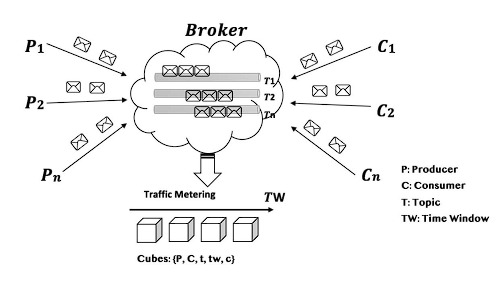
\includegraphics[width=8cm, height=6cm]{L3}
\caption{ Centralized Brokered IoT Data Marketplace Architecture}
\end{center}
\end{figure}


As opposed to IOTA, Streamer (streamr.com) felt that
there is no need to develop a completely new blockchain
and instead, saving resources by using the existing Ethereum
blockchain. It is a real time data streams exchange platform.
It creates an ecosystem for data producers to sell their data to
consumers. As explained in their white paper, a data producer
creates a data streams for their data and push it to brokers
nodes which is responsible to deliver it to its data consumer
who purchase the desired data by the interaction with the
Ethereum smart contract for management, data permission
and payment.\par
Trust and reputation management is not directly addressed
in this paper, however a trust management model should
also be established as part of the marketplace. Existing trust
frameworks can be used on top of our infrastructure. Yan et
al. , for instance, explore the notion of trust across the
IoT platform layers (physical sensing, network, and application layers), with the focus on a wide range of properties
from security to goodness, strength, reliability, availability,
ability of data. However, their survey largely overlooks issues
of trust amongst participants in a data marketplace, i.e., in the
context of data exchange transactions. More directly useful
340
in our setting, is Roman and Gatti’s study of trust in data
marketplaces , based on credit scoring, where a direct
connection is made to the use of blockchain technology with
data trading.
\\
The model consists of the following elements:\\
1) The description of data offered by a Producer;\\
2) A trade agreement, which includes details of the data
to be exchanged and the exchange protocol, the corresponding market value, and additional parameters such
as BS mentioned above;\\
3) A protocol for the exchange of data receipts, which
includes both parties in addition to a neutral smart
contract;\\
4) A reputation model, which allows a reputation score
to be assigned to every pair P and C of participants
at the end of each transaction they are involved in.
Participants may use reputation scores to assess the
risk of entering into an agreeement with an untrusted
participant.
\par
The smart contract is responsible for each transaction
associated with (1-3), and specifically for recording (i) the
specification of the data offering, (ii) the trade agreement,
and (iii) each data receipt.





\newpage
\subsubsection{Advantages}
\begin{itemize}
\item Architecture is simple.
\item Requirements are natural.

\end{itemize}
\vspace{10px}
\subsubsection{Disadvantages}
\begin{itemize}
\item Transaction is complex.
\item Ethereum cost model is too high.

\end{itemize}
\vspace{10px}





\newpage
\subsection{G2R Crypto Wallet using Indian language Mnemonics }

They present the design of a G2R Crypto Wallet
here. BIP39 uses random mnemonics. The mnemonic
library is added as a separate .bsv file. The bsv file contains
word lists from varied languages – English, Japanese,
Spanish, French, Italian, Portuguese, Russian etc. But it
does not contain any Indian language mnemonics. They have
created .bsv files for Hindi and Tamil language. In this
paper we present how Indian language mnemonics are
created and the design of a G2R crypto wallet. G2R crypto
wallet uses a random function generator and a HMAC
cocktail. This paper also justifies the choice of selection of
SRFG and Cocktail for the design of G2R crypto wallet.

\subsubsection{Introduction}

Elliptic Curve Digital Signature Algorithm (ECDSA)
with Secp256k1 is used in Bitcoin. ECDSA consists of
a pair of keys– Private key and its corresponding public
key. The public key is used with hash function and it
enables sender to send funding based on the publicly
available address. The private key is used for digitally
signing the documents to spend the funds. Validation is
possible with the public key itself.\par
 Wallet can be defined as a data structure used to store
and manage user keys. In other words, wallets do not
contain coins, but they contain keys to access the coins.
These Keys are completely independent that are created
and managed by the wallet.\par
 A hierarchical deterministic wallet  is a type of
cryptocurrency wallet that derives private keys from a
seed. It differs from non-deterministic wallet, in such a
way that it is very flexible to use, interoperable with
enhanced privacy. It has the advantage of one-time
backup. However, there was still a problem –
remembering / writing down the random string of digits of
master key.\par
 Free wallet is a cold storage wallet capable of
withdrawing from and to any cryptocurrency. Edge,
based on zero knowledge is a single sign on, one touch
two factor authentication based wallet. Atomic is a user
friendly and instant exchange custody free app.
Blockchain wallet is a hierarchical deterministic and open
source software. In copay, the group approves the
transactions and have multiple users. Jaxx is a cold
storage where verification is not required. Electrum is an
open source with address tagging and encryption feature.
Xapo is a simple bitcoin mobile wallet with added
security of a cold storage wallet. Ledger nano S, Trezor
and Keepkey are some of the hardware wallets.There are
few desktop based wallets such as Electrum, copay,
Armory, exodus etc. 
Bitcoin Improvement proposal is a design document
and may be accepted as a standard for introducing new
features or information to Bitcoin. There are three types
of BIP proposal namely Standard track BIPs,
Informational BIPs and Process BIPs.\par
 The surprise in BIP32 was that instead of creating
backup of keys, we can take a backup of a single seed.
From a given seed, we can generate unlimited private and
public keys in a deterministic fashion. 
 BIP 39 uses random mnemonics that can be converted
into master extended private keys. This mnemonic library
should be included as a separate bsv file. The bsv file
contains word lists from varied languages – English,
Japanese, Spanish, French, Italian, Portuguese, Russian
etc.

 It can be found that remembering and writing down
mnemonics is much simpler and easier to rather than the
random digits.
 BSV file exists for English, Japanese, Korean, French,
Italian, Chinese, Czech etc. It is found that no Indian
language bsv file exists and hence a mnemonic library
containing Indian languages is developed. We developed
Hindi and Tamil language mnemonics. 

\newpage
\subsubsection{Working}

G2R Algorithm:
\\
\\
Following steps are important in the design of G2R
wallet.
\\
1. Generate mnemonic phrase using Indian
language words. We have developed a list of
2048 words for Hindi and Tamil language.
Following Rules were used to create 2048 each
hindi and tamil language words.
\\o Length of the word – 4 to 10 characters
\\o Simple and Commonly used words
\\o Words can be uniquely identified using the first
4 characters
\\o No embarrassing words
\\o No words representing a particular religion
\\o No very similar words with 1 letter difference
\\o No complex verb forms
\\o No plural words
\\o No words that remind sad/bad/negative things
\\o No accents or special characters
\\o No personal or geographical names
\\o If both male and female version of words are
available, then only male version is chosen
\\o Only words starting with consonants are used
in Hindi where as in tamil words starting with
uyir mei ezhuthu are considered. In Tamil
language, the words does not start with a
consonant. Hence a uyir mei ezhuthu which is
a combination of a vowel and consonant are
considered.
\\o Words are shortlisted
\\
\\
2. PBKDF2 function is replaced with SRFG
function.

\par PBKDF2 uses a pseudorandom function. It
creates a binary seed value. HMAC SHA 512 is
used and the iteration is done for 2048 times.
This key is subsequently used a cryptographic
key for further operations. One weakness of
PBKDF2 is that, it can be realized in a small
circuit. As it requires very little random access
memory, brute-force attacks using ASICs or
GPUs become possible with less cost. Hence we
replaced PBKDF2 with SRFG. 
\\
\\
3. HMAC SHA 512 is replaced with HMAC
Cocktail 512
\par

 Hoch and Shamir considered the general
case of iterated concatenated and expanded
functions. They proved that even if we allow
each of the iterated hash function to go through
the input multiple times in an arbitrary expanded
order, their concatenation is not stronger than a
single function. Also, the authors extended their
result to tree-based hash functions with arbitrary
tree structures. They proved that the Iterated
Concatenated Expanded functions and its
generalization TCE is vulnerable to a
multicollision attack. They further believed that
the techniques they developed would help in
creating multicollision attacks against even more
complicated types of hash functions. Such a
conclusion was perhaps hinting to probable
attack on SHA 2 family of hash functions. Later
then, NIST announced SHA 3 competition and
announced Keccak as the winner.\par
 In G2R wallet, we require a simple, efficient
and flexible hash function that blends security
with speed.\par
 Cocktail, the algorithm proposed by Rajeev
Sobti,  in his thesis comes handy. Here we
will use HMAC of Cocktail.
 \par The following paragraph gives justification of
why Cocktail is applied.
\\
 Performance - Cocktail outperforms all SHA3
finalists including ‘Keccak’, the winner
announced by NIST. The comparison SHA-3
final round candidate algorithms reflects that, on
32-bit architecture (ARM as well Intel), Cocktail
is fastest among all the candidate algorithms
irrespective of whether Cocktail is used with
recommended rounds or increased rounds
(increased by 20\% for 256-bit hash and about
17\% for 512-bit hash). With recommended
rounds, Cocktail is 11\% to 45\% faster than SHA3 final round candidate algorithms depending on
hash size and processor architecture used. With
increased rounds, this margin reduces and varies
between 4\% to 23\%. On Intel 64-bit architecture,
Skein’s performance for 256-bit hash is quite
competitive. With same diffusion factor
(increased rounds of Cocktail), Skein is
marginally faster (15.49 CPB compared to 15.60
CPB) than Cocktail, but for 512-bit hash
Cocktail is the best with 8.7 CPB (16\% better
than No. 2 performer)\par
 Security - SHA-1, SHA-2 and many other
hash functions are based on Davies Meyer
scheme and hence fixed points can be easily
found for these functions. This new ARX based
hash function Cocktail makes use of Modified
ChaCha Core (MCC), to build its compression
function and output transformation. Cocktail’s
iterative structure is a variant of Matyas–Mayer–
Oseas iteration mode and uses number of
message bits hashed so far as one of the input to
compression function that makes every call to
compression function unique. Cocktail family
consists of two hash functions - Cocktail-512 and
Cocktail-1024 - that work on 32-bit and 64- bit
word size respectively and internal state is
always double the output size. Each round of
compression function is a Double round of MCC
and sub-key is injected in alternate rounds. The
key expansion is quite efficient and uses round
dependent constants. Cocktail’s compression
function can generate full diffusion in the second
round. \par The whole algorithm can be implemented
in about 350 bytes of RAM and additional 96
bytes for constants. Number of rounds is taken as
a tuneable parameter. However, to have diffusion
factor of more than five, 10 rounds for Cocktail512 and 12 rounds for Cocktail-1024 are
recommended. Decision to have ARX based
design makes it quite simple and efficient. Multirate padding, fixed initial value, and wide
internal state helps in thwarting multiple generic
attacks. The decision to have four column rounds
followed by four row rounds gives a lot of scope
to exploit parallelism. Being based on familiar
constructs that have been analysed considerably,
helps in generating more confidence in Cocktail
for its security and efficiency.\par
 The question here is why cocktail cannot be
used as it is and why HMAC is required. We
need key to generate an HMAC. The key is
shared with trusted third parties. If we only share
this key with trusted parties, given an HMAC
signature, we can be confident that only one of
the trusted parties could have generated that
signature. Thus a HMAC not only provides
collision resistance, but is also unable to be
forged. 




\newpage

\subsubsection{Advantages}
\begin{itemize}
\item It has one time backup.
\item Capable of withdrawing from and to any cryptocurrency.

\end{itemize}
\vspace{10px}
\subsubsection{Disadvantages}
\begin{itemize}
\item Creates a binary seed value.
\item Possibility of collision.


\end{itemize}
\vspace{10px}

\newpage
\subsection{Characteristics of Wallet Contracts on Ethereum
}

For the management of cryptocurrencies or cryptographic tokens, many users employ a software wallet that
facilitates the interaction with a blockchain in general or with
on-chain programs (smart contracts) in particular. While many
blockchain wallets execute their core program code off-chain,
some wallets implement core functionality on-chain as smart
contracts with the intent to increase trust and security by using
transparent and verifiable execution.
In this work, we investigate smart contracts for wallets with
regard to the functionality that makes use of cryptographically
secured blockchain technology. We focus on wallet contracts
deployed on Ethereum, as it is the most prominent platform for
tokens and smart contracts with readily available data. We aim at
a better understanding of this frequently deployed group of smart
contracts by analyzing characteristics of wallet contracts and
grouping them into six types. To this end, we present approaches
to identify wallet contracts by analyzing source code, bytecode,
and execution traces extracted from transaction data. Moreover,
we investigate usage scenarios and patterns. From the derived
data, we extract blueprints for wallets and compile a ground
truth. We provide numbers and temporal perspectives regarding
the creation and use of wallets.

\subsubsection{Introduction}


\par Wallets keep valuables, credentials, and items for access
rights (like cash, licenses, credit cards, key cards) in one place,
for ease of access and use. On the blockchain, cryptocurrencies
play a role similar to cash, while cryptographic tokens are a
universal tool for handling rights and assets. Blockchain wallets manage the cryptographic keys required for authorization
and implement the protocols for interacting with blockchains.
Smart contracts are described as a disruptive financial
technology, and crypto tokens are often termed the killer
application of smart contracts. Token and wallet contracts form
a large ecosystem with regard to the number of smart contracts
and transactions as well as market value. They already started
to change financial processes and markets.\par
Wallet contracts hold cryptocurrencies and access to tokens
and may offer advanced methods for manipulating the assets.
Simply by introducing the role of an ‘owner’ it becomes
possible to transfer all assets of a wallet contract transparently
and securely in a single transaction. More refined methods
include multi-signature wallets, which grant access only if
sufficiently many owners agree.\par
Ethereum is the major platform for smart contracts and
tokens. This paper investigates the usage and purpose of wallet
contracts on the main chain of Ethereum qualitatively as
well as quantitatively. In particular, we address the following
questions.\\
• How can deployed wallet contracts be identified from
transaction data?\\
• Regarding functionality, which types of wallet contracts
are deployed?\\
• When and in which quantities are wallets created, and
how many are actually used?\\
Methodologically, we start from available source code of
wallets and determine characteristic functions. Then we search
the deployed bytecode for variants of the wallets with the same
profile. Some wallets can also be detected by their creation
history or by the way they interact with other contracts. We
group the wallets according to their functionality and collect
creation and usage statistics from the transaction data. Finally,
we relate wallets to other frequently occurring contract types.\par
This work contributes to a better understanding of the
actual usage of smart contracts in general and wallet contracts
in particular. This may concern users, investors, companies,
developers, and regulators. To facilitate assessment, we seek
methods for detecting, classifying and monitoring the rapidly
growing ecosystem around crypto assets. Specifically, they
extract a comprehensive collection of blueprints for wallet
contracts and thereby compile a ground truth. Moreover, the
wallet blueprints and the features they implement may serve
as a resource for designing further decentralized trading apps.
For an extended version of this work see .
Roadmap: Section II clarifies terms and presents our methods for bytecode analysis. Section III discusses methods for
the identification of potential wallet contracts. Section IV
describes characteristic features of wallets and categorizes
them into types. Section V analyzes interactions of wallets.
Section VI compares our approach to related work. Finally,
section VII concludes with a summary of our results.




\newpage
\subsubsection{Working}

Ethereum [2]–[4] distinguishes between externally owned
accounts, often called users, and contract accounts or simply
contracts. Accounts are uniquely identified by addresses of
20 bytes. Users can issue transactions (signed data packages)
that transfer value to users and contracts, or that call or create
contracts. These transactions are recorded on the blockchain.
Contracts need to be triggered to become active, either by a
 transaction from a user or by a call (a message) from another
contract. Messages are not recorded on the blockchain, since
they are deterministic consequences of the initial transaction.
They only exist in the execution environment of the Ethereum
Virtual Machine (EVM) and are reflected in the execution trace
and potential state changes. We use ‘message’ as a collective
term for any (external) transaction or (internal) message.\par
Unless stated otherwise, statistics refer to the Ethereum
main chain up to block 10 000 000 (mined on May 4, 2020).
We abbreviate factors of 1 000 and 1 000 000 by the letters k
and M, respectively.\par
To a large extent, our analysis is based on the EVM
bytecode of deployed contracts. If available we use verified
source code from etherscan.io, but relying solely on
such contracts would bias the results: in contrast to 25.4 M
successful create operations, there are verified source codes
for 86.5 k addresses (0.34 \%) only.\par 
To detect functional similarities between contracts we compare their skeletons. These are obtained from the bytecodes
of contracts by replacing meta-data, constructor arguments,
and the arguments of PUSH operations uniformly by zeros
and by stripping trailing zeros. The rationale is to remove
variability that has little impact on the functional behavior,
like the swarm hashes added by the Solidity compiler or hardcoded addresses of companion contracts. Skeletons allow us
to transfer knowledge gained about one contract to others with
the same skeleton. Note that the 25.4 M contract deployments
correspond to only 280 k distinct bytecodes and 131 k distinct
skeletons. Thus, we are able to relate 11.5 M of these deployments to some source code on etherscan.io, an increase
from 0.34 to 45 \%.Most contracts in the Ethereum universe adhere to the ABI
standard [5], which identifies functions by signatures that
consist of the first four bytes of the Keccak-256 hash of the
function name and the parameter types. The bytecode of a
contract contains instructions to compare the first four bytes
of the call data to the signatures of its functions. To understand
the implemented interface of a contract, we extract it from the
bytecode, and then try to restore the corresponding function
headers.



\begin{figure}[h!]
\begin{center}
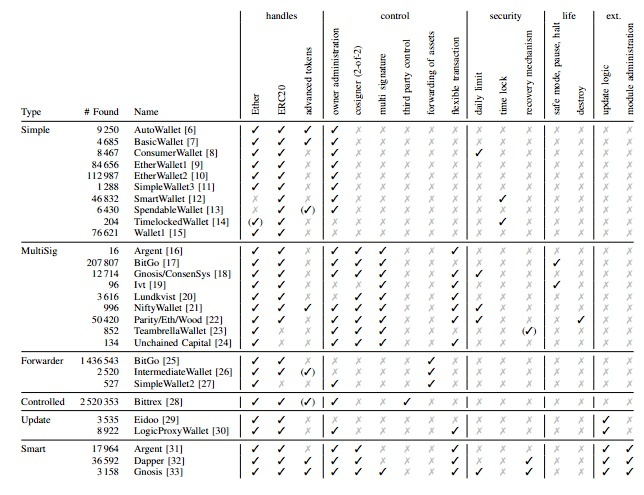
\includegraphics[width=17cm, height=13cm]{L5}
\caption{Characteristics Of Wallet Contracts}
\end{center}
\end{figure}



1) Interface Extraction: We developed a pattern-based tool
to extract the interface contained in the bytecode. As ground
truth for validation, we used the combination of verified
source code, corresponding bytecode, and ABI provided by
Etherscan. The signatures extracted by our tool differed from
the ground truth in 86 cases. Manual inspection revealed that
our tool was correct also in these cases, whereas the ABIs did
not faithfully reflect the signatures in the bytecode (e.g. due
to compiler optimization or library code).\par
Before applying the tool to all deployed bytecodes, a
few considerations are due. Apart from a small number of
LLL or Vyper contracts, the validation set consists almost
exclusively of bytecode generated by the Solidity compiler,
covering virtually all its releases (including early versions).
Regarding the large group of 11.3 M deployed contracts (259 k
codes, 130 k skeletons) generated by the Solidity compiler, the
validation set is thus representative.\par
Another interesting group of deployed contracts consists
of 9.8 M short contracts (24 k codes, only 420 skeletons)
without entry points. They are mostly contracts for storing
gas (gasToken), but also some proxies (contracts redirecting
calls elsewhere) and contracts involved in attacks. A third large
group are 4.2 M contracts that self-destruct at the end of the
deployment phase (mayflies [35]). They cannot be regularly
called and thus do not contain any entry points either.\par
What remains are 1.4 k contracts (595 codes). For them,
our tool shows an error rate of 8 \%, estimated from a random
sample of 60 codes that we manually checked.\\

\par2) Interface Restoration: To understand the purpose of
contracts we try to recover the function headers from the
signatures. As the signatures are partial hashes of the headers,
we use a dictionary of function headers with their 4-byte
signatures (collected from various sources), which allows us to
obtain a function header for 58\% of the 294 k distinct signatures on the main chain.2 Since signatures occur with varying
frequencies and codes are deployed in different numbers, this
ratio increases to 90 \% (or 89 \%) when picking a code (or a
deployed contract) at random.
\\
\\
The identified 28 variants of proper wallets (blueprints)
differ in functionality and number of deployments. Based on
their features, we assign them to one of six groups.\\
1) Simple Wallets: provide little extra functionality beyond
handling Ether and tokens. A sample can be found at [12].\\
2) MultiSig Wallets: require that m out of n owners sign a
transaction before it is executed. Usually the required number
of signatures (m) is smaller than the total number of owners
(n), meaning that not all owners have to sign. In most cases,
the set of owners and the number of required signatures can
be updated.\\
3) Forwarder Wallets: forward the assets they receive to
some main wallet. They may include owner management.
BitGo employs large numbers of forwarder wallets in combination with its variant of a multiSig wallet [17].\\
4) Controlled Wallets: can be compared to traditional bank
accounts. They are assigned to customers, who can use them
as target of transfers, but the control over the account remains
with the bank. Withdrawals are executed by the bank on
behalf of the customer. This construction allows to comply
with legal regulations that may restrict transactions. Regarding
the number of deployments, controlled wallets are the most
common type.\\
5) Update Wallets: provide a mechanism to update their
main features at the discretion of the owner. A sample can be
found at [29], [30]\\
6) Smart Wallets: offer enhanced features like authorization
mechanism for arbitrary transactions, recovery mechanisms for
lost keys, modular extension of features, or advanced token
standards.
\par they examine the usage of wallets, differentiate token holdings, and discuss the role of wallets within the
smart contracts landscape.\\
The 10 M blocks of the Ethereum main chain contain
697.4 M transactions, which gave rise to 1 761 M messages
and 25.4 M successfully created contracts. About 4.66 M of
them (18.4 \%) are wallets. The wallets received 28.2 M and
sent 54.0 M calls, with 2.8 M inter-wallet calls. In total, 85.0 M
messages (4.8 \%) involve wallets.



\newpage
\subsubsection{Advantages}
\begin{itemize}
\item Wallets keep valuables and other aspects in one place.
\item Wallet contracts hold cryptocurrencies.

\end{itemize}
\vspace{10px}
\subsubsection{Disadvantages}
\begin{itemize}
\item Messages are not recorded on the block chain.
\item There only exists the execution environment of Ethereum.

\end{itemize}
\vspace{10px}













\newpage























\begin{flushleft}\textbf{CHAPTER 3} \end{flushleft}
\begin{flushleft}\section{TECHNOLOGIES USED } \end{flushleft}

\vspace*{10px}
\subsection{Model–view–viewmodel}
Model–view–viewmodel (MVVM) is a software architectural pattern that facilitates the separation of the development of the graphical user interface (the view) – be it via a markup language or GUI code – from the development of the business logic or back-end logic (the model) so that the view is not dependent on any specific model platform. The viewmodel of MVVM is a value converter, meaning the viewmodel is responsible for exposing (converting) the data objects from the model in such a way that objects are easily managed and presented. In this respect, the viewmodel is more model than view, and handles most if not all of the view's display logic. The viewmodel may implement a mediator pattern, organizing access to the back-end logic around the set of use cases supported by the view.
\\
\\
\textbf {Model}
\par 
Model refers either to a domain model, which represents real state content (an object-oriented approach), or to the data access layer, which represents content (a data-centric approach).
\\
\textbf{View}
\par
As in the model–view–controller (MVC) and model–view–presenter (MVP) patterns, the view is the structure, layout, and appearance of what a user sees on the screen. It displays a representation of the model and receives the user's interaction with the view (mouse clicks, keyboard input, screen tap gestures, etc.), and it forwards the handling of these to the view model via the data binding (properties, event callbacks, etc.) that is defined to link the view and view model.
\\
\textbf{View model}
\par
The view model is an abstraction of the view exposing public properties and commands. Instead of the controller of the MVC pattern, or the presenter of the MVP pattern, MVVM has a binder, which automates communication between the view and its bound properties in the view model. The view model has been described as a state of the data in the model.\par
The main difference between the view model and the Presenter in the MVP pattern is that the presenter has a reference to a view, whereas the view model does not. Instead, a view directly binds to properties on the view model to send and receive updates. To function efficiently, this requires a binding technology or generating boilerplate code to do the binding.
\\
\textbf{Binder}
\par
Declarative data and command-binding are implicit in the MVVM pattern. In the Microsoft solution stack, the binder is a markup language called XAML. The binder frees the developer from being obliged to write boiler-plate logic to synchronize the view model and view. When implemented outside of the Microsoft stack, the presence of a declarative data binding technology is what makes this pattern possible, and without a binder, one would typically use MVP or MVC instead and have to write more boilerplate (or generate it with some other tool).

\subsection{Application Programming Interface}


An application programming interface (API) is a connection between computers or between computer programs. It is a type of software interface, offering a service to other pieces of software. A document or standard that describes how to build or use such a connection or interface is called an API specification. A computer system that meets this standard is said to implement or expose an API. The term API may refer either to the specification or to the implementation.\par
In contrast to a user interface, which connects a computer to a person, an application programming interface connects computers or pieces of software to each other. It is not intended to be used directly by a person (the end user) other than a computer programmer who is incorporating it into the software. An API is often made up of different parts which act as tools or services that are available to the programmer. A program or a programmer that uses one of these parts is said to call that portion of the API. The calls that make up the API are also known as subroutines, methods, requests, or endpoints. An API specification defines these calls, meaning that it explains how to use or implement them.\par

One purpose of APIs is to hide the internal details of how a system works, exposing only those parts a programmer will find useful and keeping them consistent even if the internal details later change. An API may be custom-built for a particular pair of systems, or it may be a shared standard allowing interoperability among many systems.

\subsection{Combine}


The Combine framework provides a declarative Swift API for processing values over time. These values can represent many kinds of asynchronous events. Combine declares publishers to expose values that can change over time, and subscribers to receive those values from the publishers.\par
The Publisher protocol declares a type that can deliver a sequence of values over time. Publishers have operators to act on the values received from upstream publishers and republish them.

At the end of a chain of publishers, a Subscriber acts on elements as it receives them. Publishers only emit values when explicitly requested to do so by subscribers. This puts your subscriber code in control of how fast it receives events from the publishers it’s connected to.

You can combine the output of multiple publishers and coordinate their interaction. For example, you can subscribe to updates from a text field’s publisher, and use the text to perform URL requests. You can then use another publisher to process the responses and use them to update your app.

By adopting Combine, you’ll make your code easier to read and maintain, by centralizing your event-processing code and eliminating troublesome techniques like nested closures and convention-based callbacks.






\newpage
\begin{flushleft}\textbf{CHAPTER 4} \end{flushleft}
\begin{flushleft}\section{SOFTWARE REQUIREMENTS\&
HARDWARE REQUIREMENTS} \end{flushleft}
\vspace*{10px}
\subsection{SOFTWARE REQUIREMENTS}

\begin{itemize}
\item Operating System             \hspace{21.5mm}: \hspace{19mm}   Mac os Monterey
\item Programming Language               \hspace{10.5mm}: \hspace{20mm}   Swift 
\item Framework\hspace{35mm}: \hspace{19mm}  API
 \item IDE                      \hspace{46mm}: \hspace{20mm} Xcode
\end{itemize}
\vspace{10px}
       
\subsection{HARDWARE REQUIREMENTS}

\begin{itemize}
\item Processor      \hspace{23mm}: \hspace{20mm}    2.3GHz dual-core Intel Core i5
\item Primary Memory    \hspace{9mm}: \hspace{20mm}  8GB RAM and above                
\item Storage    \hspace{26.5mm}: \hspace{20mm}    256 GB Hard Disk and above
 \item Display     \hspace{26.5mm}: \hspace{20mm}   Retina display 
\item Key Board  \hspace{20.5mm}: \hspace{20mm}           Mac compatible 
\item Trackpad        \hspace{23mm}: \hspace{21.5mm}Mac Compatible 
\end{itemize}
\vspace{10px}





\newpage
\begin{flushleft}\textbf{CHAPTER 5} \end{flushleft}
\begin{flushleft}\section{SYSTEM DESIGN} \end{flushleft}
\vspace*{10px}

\subsection{Data Flow Diagram}

The data flow diagram (DFD) is one of the most important tools used by system
analyst. Data flow diagrams are made up of a number of s ymbols, which represent
system components. Most data flow modelling methods use four kind of symbols.
These s ymbols are used to four kinds of system components. Processes, data source,
data flow and external entities. 
Processes are represented by circles in DFD.Dataflow represented by a thin
line in the DFD and each data store has a unique name and square or represents
external entities unlike detailed flow chart, data flow diagram do not supply detailed
description of the modules but graphically describes a systems data and how the data
interact with the system.
To construct a data flow diagram the following symbols are used:


\begin{figure}[h!]
\begin{center}
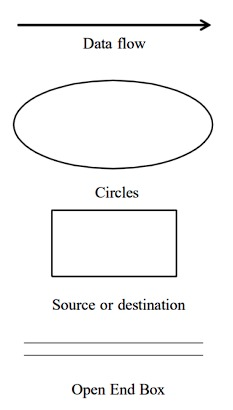
\includegraphics[width=5cm, height=8cm]{DFD}
\caption{symbols}
\end{center}
\end{figure}

\newpage

\par An arrow identifies the data flow in motion. It is a pipe line through which
information is flown like the rectangle in the flow chart. A circle stands for process that
converts data into information's. An open-ended box represents a data store, data at rest
or a temporary repository of data. A square defines a source or destinations of system
data.

\begin{flushleft}\textbf{Level 0}\end{flushleft}


\begin{figure}[h!]
\begin{center}
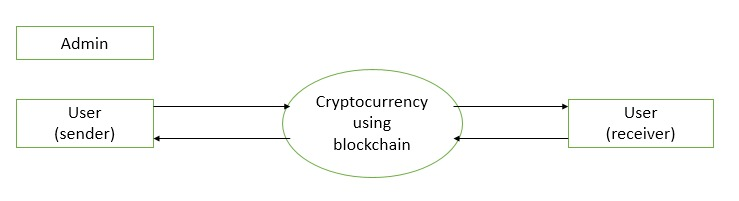
\includegraphics[width=17cm, height=5cm]{DFD1.0}
\caption{level 0 DFD}
\end{center}
\end{figure}
\newpage

\begin{flushleft}\textbf{Level 1.1}\end{flushleft}


\begin{figure}[h!]
\begin{center}
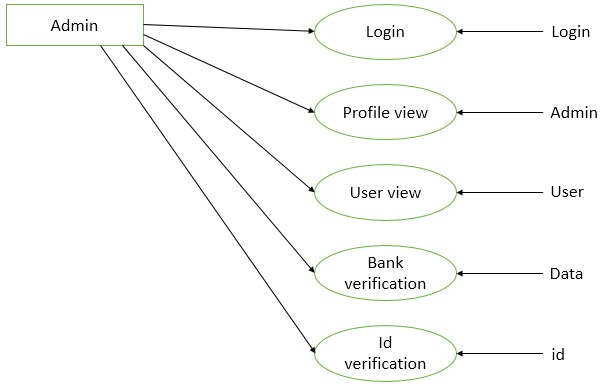
\includegraphics[width=16cm, height=9cm]{DFD1.1}
\caption{ level 1.1 DFD}
\end{center}
\end{figure}
\newpage




\begin{flushleft}\textbf{Level 1.2}\end{flushleft}


\begin{figure}[h!]
\begin{center}
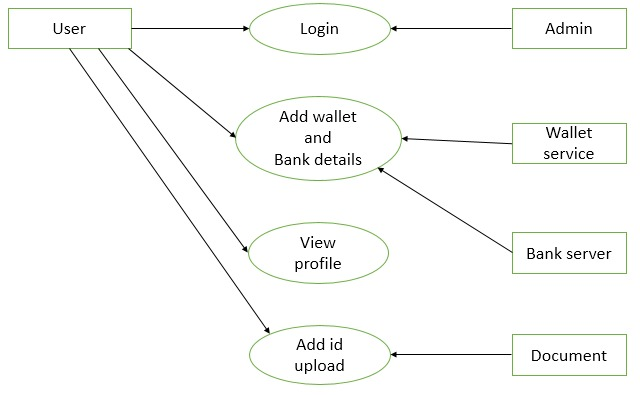
\includegraphics[width=16cm, height=9cm]{DFD1.2}
\caption{level 1.2 DFD}
\end{center}
\end{figure}








\newpage





\subsection{UML DIAGRAM}

\subsubsection{Sequence Diagram}

A sequence diagram is an interaction diagram that emphasis the time
ordering of the messages; a collaboration diagram is an interaction diagram that
emphasizes the structural organization of the objects that send and receive messages.
Sequence diagrams and collaboration diagrams are isomorphic, meaning that you
can take one and transform it into the other. Sequence diagrams are typically
associated with use case realizations in the logical view of the system under
development. Sequence diagrams are sometimes called event diagrams or event
scenarios. A sequence diagram shows, as parallel vertical lines, different processes or
objects that lives simultaneously, and as horizontal arrow, the messages exchanged
between them, in the order in which they occur. This allows the Specification of
Simple’s Runtime Scenarios In A Graphical Manner.A sequence
diagram or system sequence diagram (SSD) shows object interactions arranged in time
sequence in the field of software engineering. It depicts the objects involved in the scenario and the sequence of messages exchanged between the objects needed to carry out
the functionality of scenario. Sequence diagrams are typically associated with use case
realizations in the logical view of the system under development. Sequence diagrams
are sometimes called event diagrams or event scenarios.For a particular scenario of a
use case, the diagrams show the events that external actors generate, their order, and
possible inter-system events. All systems are treated as a black box; the diagram places
emphasis on events that cross the system boundary from actors to systems. A system
sequence diagram should be done for the main success scenario of the use case, and
frequent or complex alternative scenarios.


\begin{figure}[h!]
\begin{center}
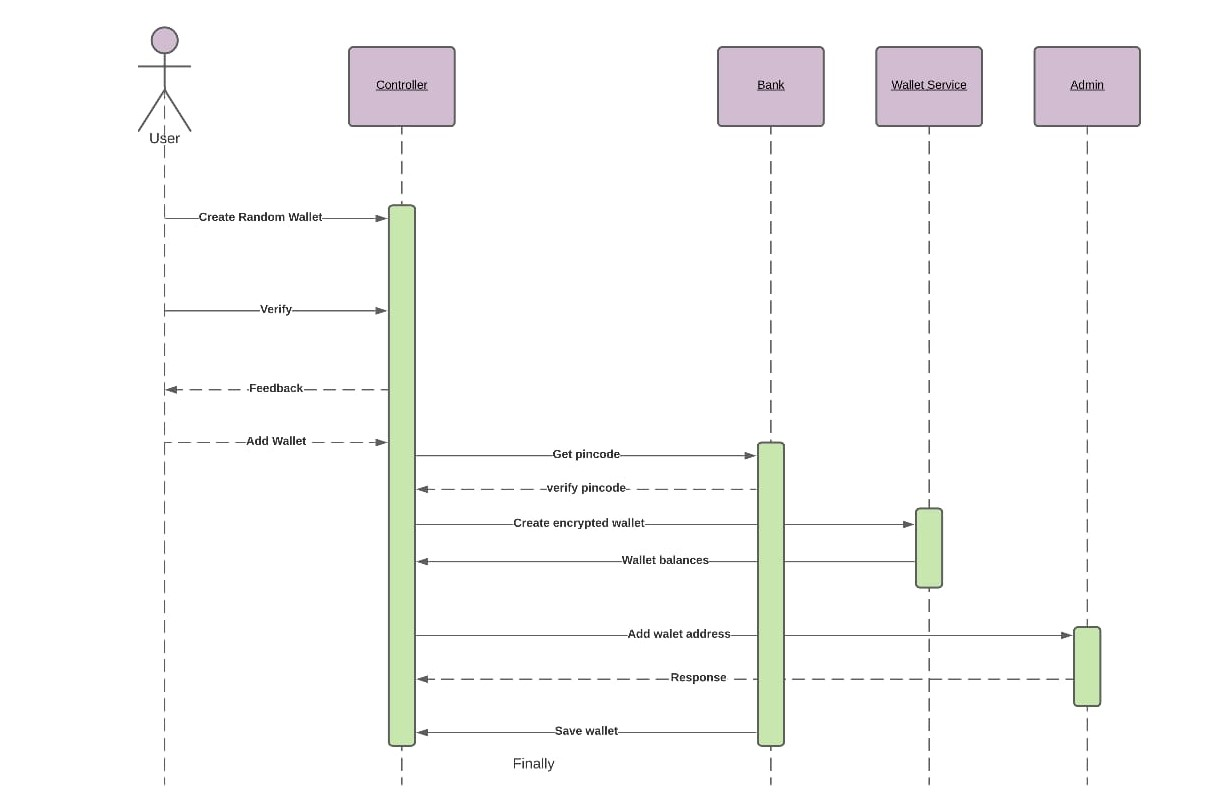
\includegraphics[width=17cm, height=9cm]{SEQ}
\caption{Sequence Diagram}
\end{center}
\end{figure}

\newpage
\subsubsection{Use Case Diagram}

A use case diagram is a graphic depiction of the interactions among the
elements of a system. A use case is a methodology used in system analysis
to identify, clarify and organize system requirements’ use case diagram at its
simplest is representation of a user's interaction with the system that shows the
relationship between the user and the different use cases in which the user is
involved. A use case diagram can identify the different types of users of a system
and the different use cases and will often be accompanied by other types of
diagrams as well.
\par The purpose of use case diagram is to capture the dynamic aspect of a
system. Use case diagrams are used to gather the requirements of a system
including internal and external influences. These requirements are mostly design
requirements. So when a system is analyzed to gather its functionalities use case
are prepared and actors are identified.


\begin{figure}[h!]
\begin{center}
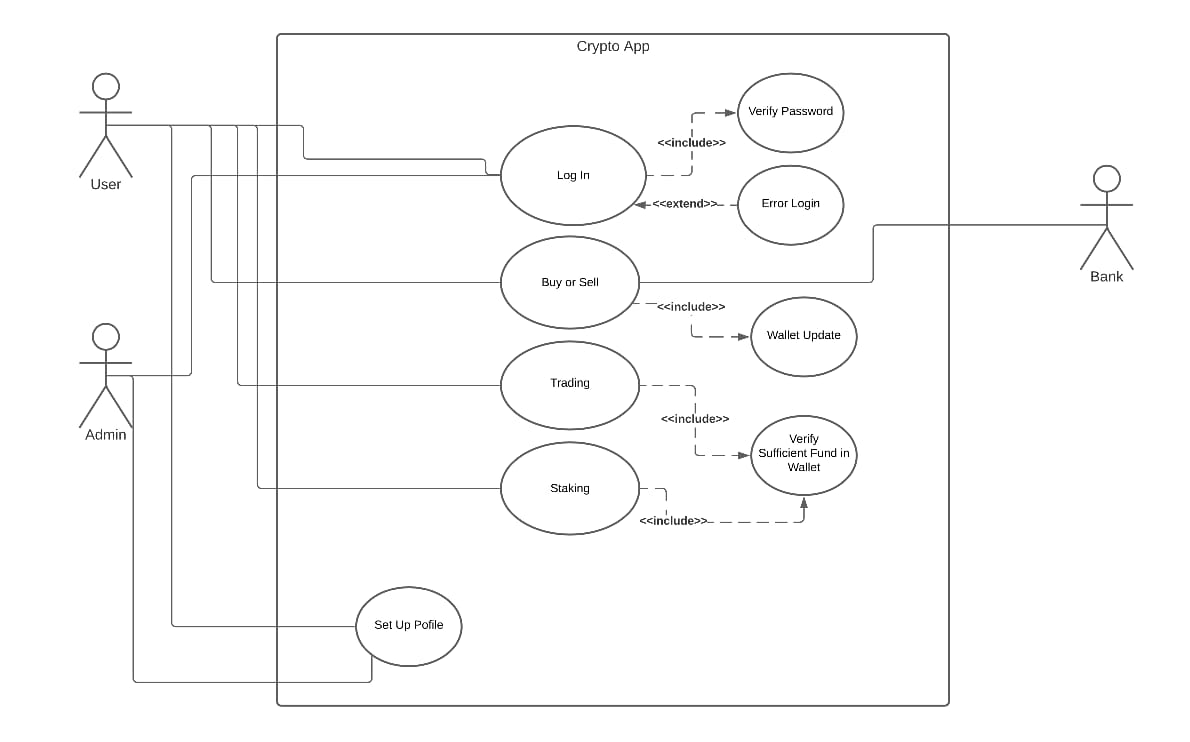
\includegraphics[width=17cm, height=11cm]{USE}
\caption{Use Case Diagram}
\end{center}
\end{figure}



\subsubsection{Activiy Diagram}


Activity diagrams are graphical representations of workflows of stepwise
activities and actions with support for choice, iteration and concurrency. In the
Unified Modelling Language, activity diagrams are intended to model both
computational and organizational processes (i.e. workflows). Activity diagrams
show the overall flow of control. Activity diagrams are constructed from a limited
number of shapes, connected with arrows. The most important shape types:
\\
\\
• Rounded rectangles represent actions;\\
\\
• Diamonds represent decisions;\\
\\
• Bars represent the start (split) or end (join) of concurrent activities;\\
\\
• A black circle represents the start (initial node) of the workflow; An encircled
black circle represents the end (final node).\\
\\
\par Arrows run from the start towards the end and represent the order in
which activities happen. Activity diagrams may be regarded as a form of
flowchart. Typical flowchart techniques lack constructs for expressing concurrency.
However, the join and split symbols in activity diagrams only resolve this
for simple cases; the meaning of the model is not clear when they are arbitrarily
combined with decisions or loops.

\newpage
\vspace*{10px}
\begin{figure}[h!]
\begin{center}
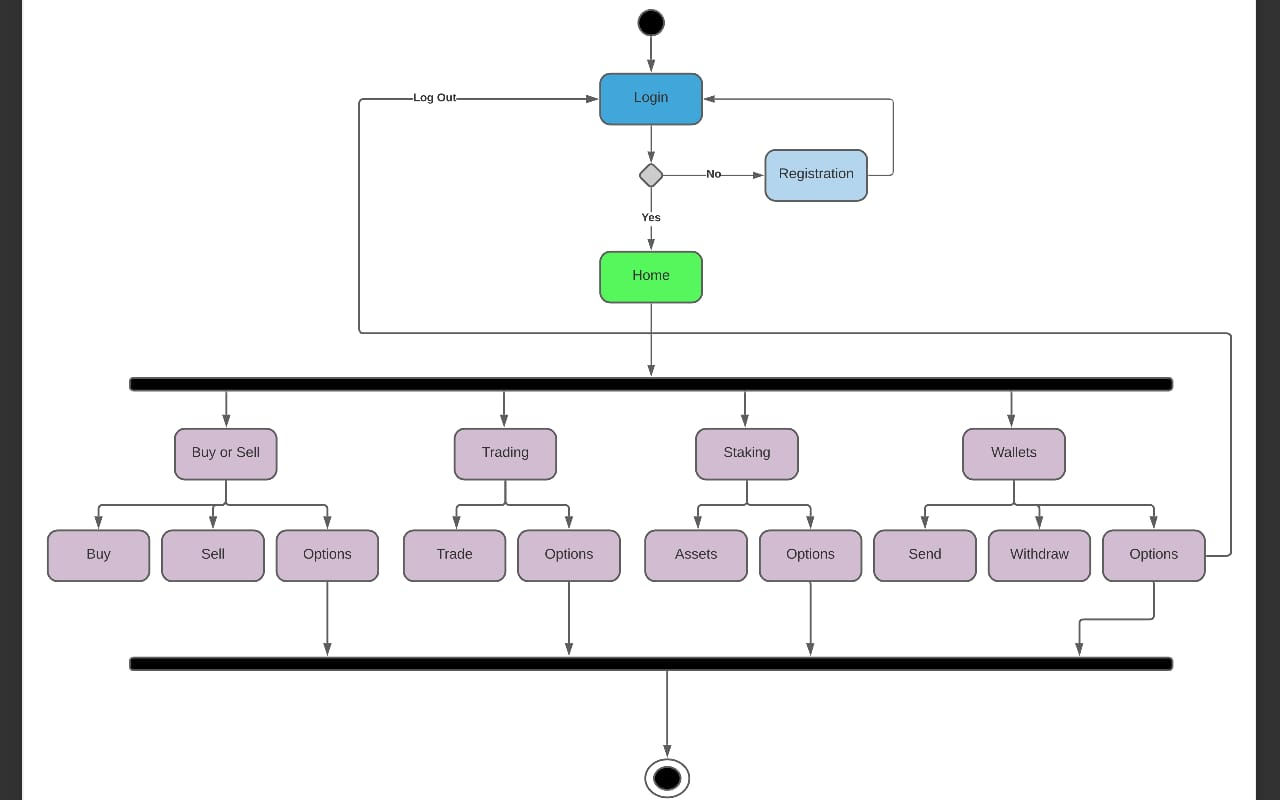
\includegraphics[width=17cm, height=11cm]{ACT}
\caption{Activity diagram }
\end{center}
\end{figure}


\newpage

\subsubsection{Class Diagram}

The class diagram is the main building block of object-oriented modelling. It is used for general conceptual modelling of the structure of the application, and for detailed modelling, translating the models into programming code. Class diagrams can also be used for data modelling.
\par Class diagram is a static diagram. It represents the static view of an application. Class diagram is not only used for visualizing, describing, and documenting different aspects of a system but also for constructing executable code of the software application. Class diagram describes the attributes and operations of a class and also the constraints imposed on the system. The class diagrams are widely used in the modeling of objectoriented systems because they are the only UML diagrams, which can be mapped directly with object-oriented languages.
\par Class diagram shows a collection of classes, interfaces, associations, collaborations, and constraints. It is also known as a structural diagram.

\begin{figure}[h!]
\begin{center}
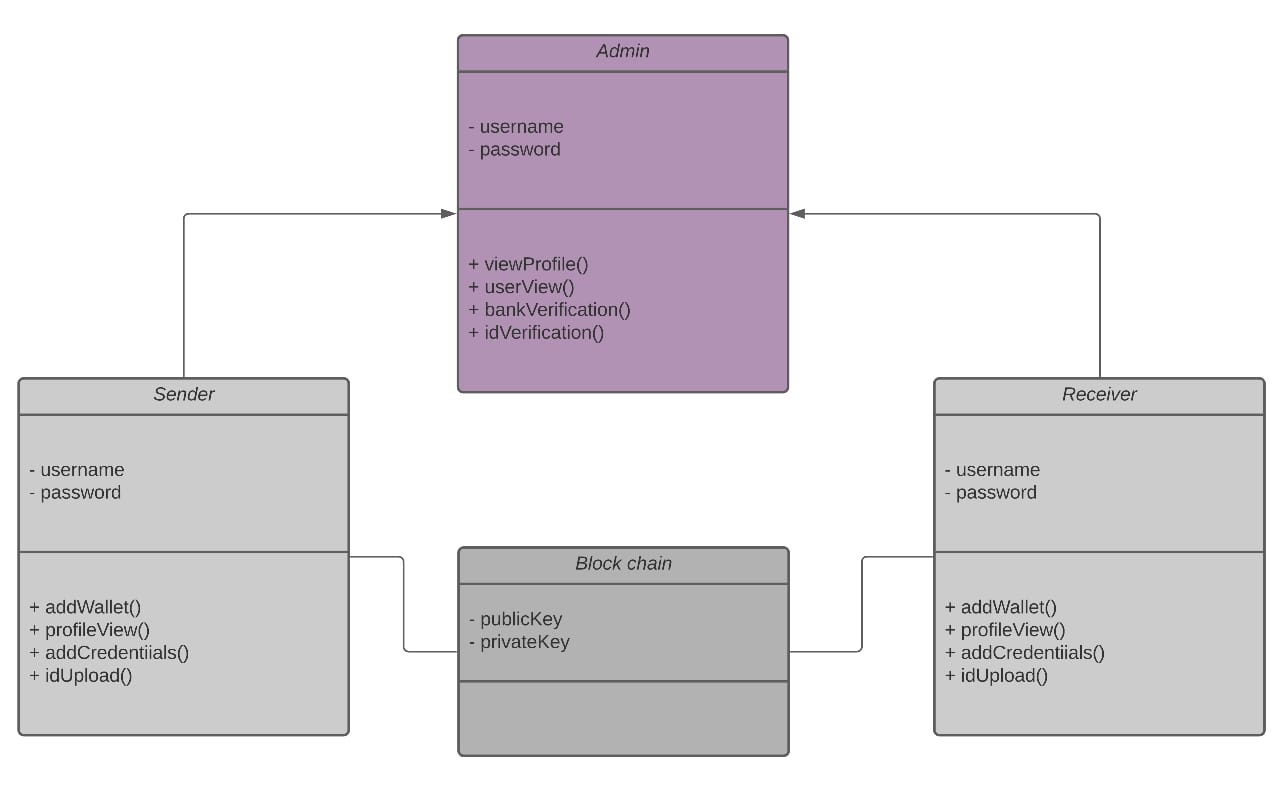
\includegraphics[width=17cm, height=10cm]{CLS}
\caption{Class Diagram}
\end{center}
\end{figure}
\newpage









\begin{flushleft}\textbf{CHAPTER 6} \end{flushleft}
\begin{flushleft}\section{CONCLUSION} \end{flushleft}

      There are plenty of wallets that are available for use. We
have selected a few sample wallets from different
categories. Most probably, all wallets use SHA256,
ECDSA key generation algorithms as they are built for
existing blockchains. Wallets such as Guarda, Jaxx
supports web, mobile and desk-top platforms. If protection
is the concern, choose a hardware wallet. If comfort is the
concern, choose an internet or cell wallet.\par
When choosing the best cryptocurrency wallets, we recommend you to make use of 2 types of wallets, a web-based
wallet and a hardware wallet. On the web-based wallet, you
store your petty cash, and on the hardware wallet, you store
all your other cryptos. Via the web-based wallet, you’ll be
trading to and fro other exchange based wallets, and then
transferring trading profits from your web-wallet onto your
hardware wallet for long term safekeeping.\par
From our limited set of sampling of wallets, i) Jaxx and
Guarda are the better choices for the web based
cryptocurrency wallets, ii) Coinomi is the best mobile
wallet, iii) Atomic Wallet is the best desktop wallet, and iv)
Ledger Nano S is the best hardware wallet. Before choosing
a cryptocurrency mobile wallet, one needs to take into
account the OS it supports, level of security as well as
supported coins. And keep in mind not to hold all your
assets in one place. It should be noted that there’s -no one
size fits all- wallet.




\newpage
\renewcommand{\thepage}{}
\begin{center}

\end{center}
\addcontentsline{toc}{section}{REFERENCES}
     \begin{thebibliography}{99}
\bibitem{title}
 Corina Sas, Irni Eliana Khairuddin, Exploring Trust in Bitcoin
Technol-ogy: A Framework for HCI Research, ACM 2015. 

\bibitem{second}
Stanislaw Jarecki, Aggelos Kiayias, Hugo Krawczyk and Jiayu Xu,
Highly Efficient and Composable Password-Protected Secret Sharing
(Or: How to Protect Your Bitcoin Wallet Online) IEEE 2016. 

\bibitem{third}
Nelisiwe Peaceness DLAMINI , Mfundo Shakes SCOTT, Kishor
Krish-nan NAIR, Development of an SMS System Used to Access
Bitcoin Wallets, IST Africa 2017. 
\bibitem{fourth}
Mahesh Shirole, Maneesh Darisi, Sunil Bhirud, Cryptocurrency
Token:An Overview, In proceedings of IC-BCT 2019
SpringerInternational Conference on Blockchain Technology,
Springer 2019. 

\bibitem{fifth}
Yi Liu, Xingtong Liu, Lei Zhang, Chaojing Tang and Hongyan Kang,
An Efficient Strategy to Eliminate Malleability of Bitcoin Transaction,
IEEE 2017. 
\bibitem{sixth}
Arunmozhi Manimuthu, Raja Sreedharan V , Rejikumar G and Drishti
Marwaha, A literature review on Bitcoin: Transformation of crypto
currency into a global phenomenon, IEEE 2018. 


\end{thebibliography}
\end{document}




































